\documentclass{article}
\usepackage{graphicx}

\title{Primes and Yitang Zhang}
\author{Owen Xuan}

\begin{document}

\maketitle
% Thank you for the feedback! :D

Prime numbers: the atoms of mathematics. Though easy to describe, primes are frustratingly hard to consistently find, yet are extremely useful. This has led to the creation of many theorems regarding the distribution of primes, the most famous of which are the twin primes conjecture and the Riemann hypothesis. Prestigious groups of Ivy League tenured professors have worked in tandem for decades trying to make a breakthrough on these two seemingly immovable problems. In all likelihood, a breakthrough in these conjectures would have come from a familiar face in the math community – but it didn’t.

Before we explore the particulars of prime numbers, it’s natural to ask why we should care about them. Prime numbers build the backbone for number theory, and are of utmost usefulness to number theorists. Perhaps surprisingly, prime numbers also play a significant role in an entirely different subject: cryptography. It turns out that the reason prime numbers are so hard to analyze – their randomness – provides cyber-age security to the internet. Most of our encrypted messages are encrypted using RSA, which relies on the fact that while computers can rapidly multiply two primes, it’s extremely difficult to do the reverse: to take an enormous number (often hundreds of thousands of digits long) and factor it. The specifics of public-private key encryption, the branch that RSA falls under, can be found here. Every time you buy something online, you're using primes.

Euclid didn't do much online shopping. He, and other mathematicians interested in primes, were instead intrigued by how they described the rest of the numerical universe. In pure mathematics, primes are often referred to as the “atoms” of mathematics; all other numbers are assembled from these principal elements. After mathematicians started playing around with primes, they began to discover all sorts of theorems, starting with Euclid’s elegant proof of the infinitude of prime numbers: if there are a finite set of prime numbers, then the number formed by multiplying all the primes in that set and adding one is divisible by none of those primes, meaning it is a prime – thus our assumption that there are only a finite set of primes is false. Commonly known theorems that have resulted from the analysis of primes include Fermat’s little theorem, Fermat’s last theorem, the Chinese Remainder Theorem, and Wilson’s theorem.

Amid this branch of literature, the crown jewels of proofs have resulted from studying the distribution of prime numbers– primarily, the prime number theorem and twin prime conjecture. We’ve already seen an estimation of the distribution of primes! Euclid’s proof of the infinite number of primes is sufficient to show that the number of primes below $n^n$ is at least $n$. This is a very loose guess, though, and mathematicians since have significantly tightened estimations. As alluded to earlier, the prime number theorem estimates the number of primes below a certain number. It states that

\[
\pi (n) \sim \frac n{\ln n}
\]
with $\pi(n)$ denoting the number of primes below $n$, which is a much more accurate prediction. 

Mathematicians also ask a different question: of the infinite amount of primes, how many differ by only two? Observing small primes, we find that amongst the numbers below twenty, there are four sets of twin primes: $(3, 5)$, $(5, 7)$, $(11, 13)$, and $(17, 19)$. However, pairs of twin primes become increasingly sparse as $n$ becomes very large. It’s natural to then wonder whether there are a finite or infinite number of twin primes. Thus borne the twin prime conjecture, first proposed in 1846, which states that there are an infinite amount of twin primes. As of today, it is still unproven. However, a less strict variant of the question has been proven, called the bounded gaps theorem. If we forget two as a constant, is there any finite (or “bounded”) number for which there are an infinite number of pairs of primes whose difference (or “gap”) is that finite number?

In 2013, amidst the bustle of well-known professors and the tenured mathematician community working toward a proof, an unknown figure experienced much more than 15 minutes of fame when he announced an astounding proof of the infamous conjecture. Yitang Zhang, a naturally quiet and reflective person with little inclination toward fame, was suddenly thrust into an interview-filled celebrity status. 

Fifty-eight at the time of the paper's publication and a former Subway employee, Zhang was an unlikely candidate for a few reasons. First, he wasn’t immersed in the math community – though Zhang earned a Ph.D. from Purdue, he left Purdue at odds with and without the support of his advisor. Due to this, and the fact that his first paper would only come in 2001 (ten years later), Zhang was unable to find an academic job. He drifted for eight years, finding odd Subway jobs or working as an accountant, before obtaining a position as a lecturer at UNH. As such, Zhang didn’t have access to a network of other specialized mathematicians – his work was mostly individual and under the radar. Second, Zhang was fifty-eight at the time of publication, far past the perceived expiration date for genius. Mathematician G. H. Hardy once wrote that he did “\dots not know of an instance of a major mathematical advance initiated by a man past fifty.” These factors made it all the more awing that Zhang discovered the proof of this 150-year-old open conjecture.

\begin{center}
    \footnotesize
    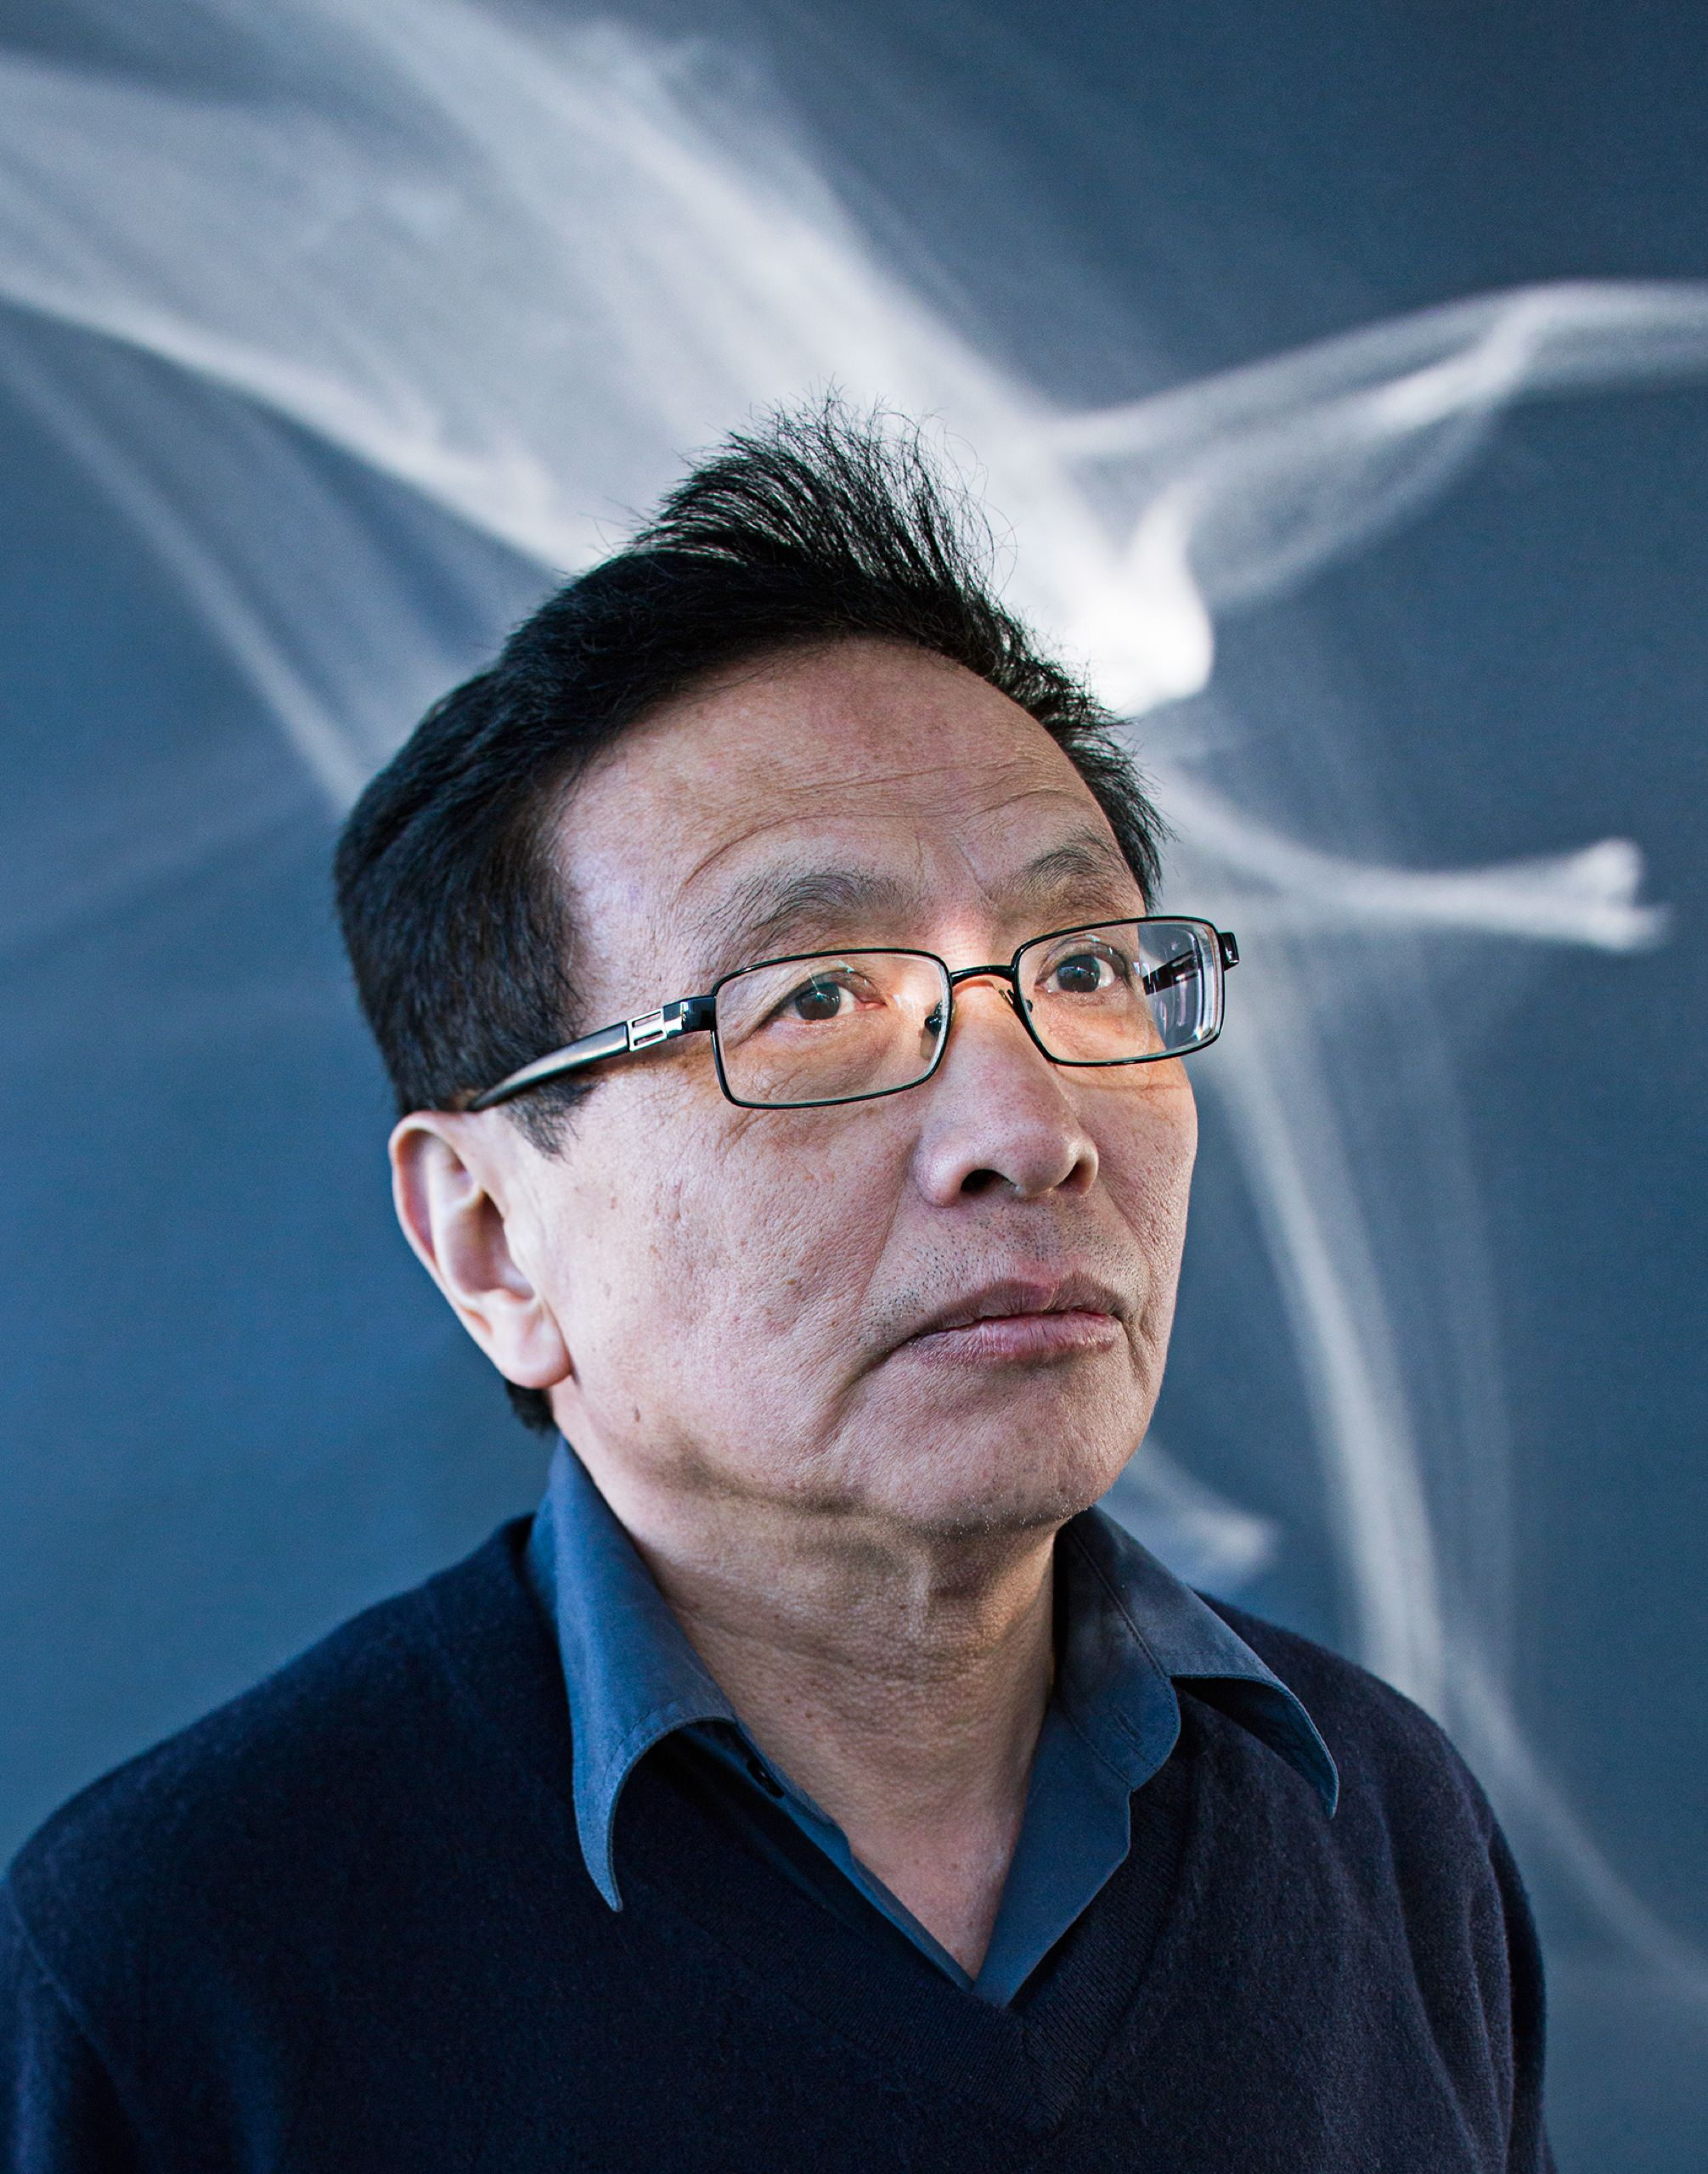
\includegraphics[scale = 0.06]{Magazines/img/Vol5/yitang.jpg}
    
    \textit{Portrait of Yitang Zhang by Peter Bohler}
\end{center}

Seventy million is a far cry from two. Though the bounded gaps theorem was finally proven, novel ideas were needed to lower the bound. In response, the mathematics community quickly came together to expedite the journey from $70,000,000$ to $2$. A forum named Polymath8 by Fields Medal recipient Terence Tao was created to improve Zhang’s bound. Excitement grew tangible as mathematicians clamored to join the project. Eventually, through a series of dependent and independent events*, the bound fell to $246$ – which becomes a startling six if another prime distribution conjecture called the Elliott-Halberstam conjecture is assumed true. 

Yitang’s legendary journey hasn’t stopped there. In November 2022, he published a new breakthrough work also related to the distribution of prime numbers, leading some to equate his success to being struck twice by lightning. His newest breakthrough is considered a major step on the path to a proof of the Riemann hypothesis – widely considered the most important unsolved problem in pure mathematics, and tying together almost every area of math. The specifics of Zhang’s new results on Landau-Siegel zeroes, which implements a generalized version of the Riemann zeta function known as the Dirichlet L-function, lies outside the scope of this article. As with his first discovery, Zhang’s second result has breathing space for improvement. After his paper is peer-reviewed and deemed accurate, some speculate another Polymath project will be created to advance Zhang’s techniques.
\end{document}